\documentclass[aspectratio=169,11pt]{beamer}
\usepackage[T1]{fontenc}
\usepackage{lmodern,amsmath,amssymb,mathtools,bm,booktabs,array,graphicx,tikz}
\usetikzlibrary{arrows.meta,positioning,calc,decorations.pathreplacing,patterns}
\definecolor{ink}{HTML}{17344D}\definecolor{accent}{HTML}{087E8B}\definecolor{pale}{HTML}{EDF5F5}\definecolor{gold}{HTML}{AD6B19}
\providecommand{\dd}{\,\mathrm{d}}\providecommand{\R}{\mathbb{R}}
\providecommand{\E}{\mathbb{E}}\providecommand{\Var}{\operatorname{Var}}
\providecommand{\Cov}{\operatorname{Cov}}\providecommand{\diag}{\operatorname{diag}}
\providecommand{\norm}[1]{\left\lVert#1\right\rVert}
\providecommand{\abs}[1]{\left|#1\right|}
\usefonttheme{professionalfonts}
\setbeamercolor{normal text}{fg=black,bg=white}
\setbeamercolor{frametitle}{fg=ink,bg=white}
\setbeamercolor{title}{fg=ink}\setbeamercolor{structure}{fg=accent}
\setbeamercolor{block title}{fg=ink,bg=pale}\setbeamercolor{block body}{fg=black,bg=pale!40}
\setbeamercolor{alerted text}{fg=accent}
\setbeamerfont{frametitle}{size=\Large,series=\bfseries}
\setbeamerfont{title}{size=\LARGE,series=\bfseries}
\setbeamertemplate{navigation symbols}{}
\setbeamersize{text margin left=.7cm,text margin right=.7cm}
\setbeamertemplate{frametitle}{\vspace{.18cm}\insertframetitle\par\vspace{.1cm}{\color{accent}\hrule height .6pt}\vspace{.12cm}}
\newcommand{\notestarget}{notes.pdf}\newcommand{\noteslabel}{Notes}
\setbeamertemplate{footline}{\hspace{.7cm}\color{ink}\scriptsize Mathematical Modeling\quad\href{\notestarget}{\noteslabel}\hfill\insertframenumber\,/\,\inserttotalframenumber\hspace{.7cm}\vspace{.18cm}}
\setbeamercovered{invisible}
\hypersetup{pdfauthor={Zan Ahmad},pdftitle={Population transfers: SIR dynamics, thresholds, and numerical conservation},pdfpagemode=UseNone}
\begin{document}
\begin{frame}[plain]\vfill
{\small\color{accent} Mathematical Modeling \quad Lecture 6}\par\medskip
{\raggedright\hyphenpenalty=10000\exhyphenpenalty=10000\LARGE\bfseries\color{ink} Population transfers: SIR dynamics, thresholds, and numerical conservation}\par\bigskip
Zan Ahmad\par\smallskip
{\small Fall 2024}\par\vfill\end{frame}
\renewcommand{\notestarget}{notes.pdf\#note-population-categories-and-contact-assumptions}
\begin{frame}[t,fragile,label=slide-a-closed-population-with-three-states]{A closed population with three states}
\[S+I+R=N.\] Susceptible, infectious, and recovered are mutually exclusive categories.\pause{}\par\medskip Recovery retains people inside the population; it removes infectiousness, not population mass.
\end{frame}
\renewcommand{\notestarget}{notes.pdf\#note-population-categories-and-contact-assumptions}
\begin{frame}[label=slide-homogeneous-mixing-and-infection-flux-figure]{Homogeneous mixing and infection flux}
\centering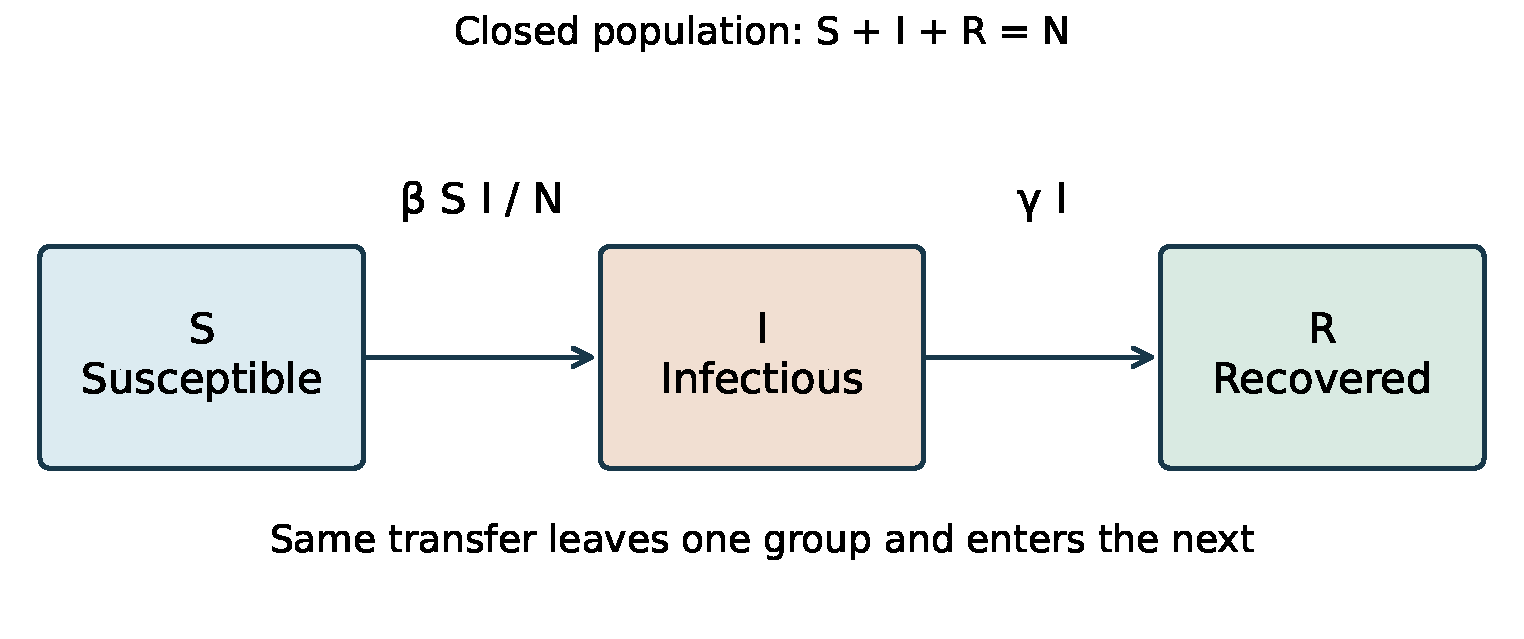
\includegraphics[width=.98\linewidth,height=.69\textheight,keepaspectratio]{population-transfers.pdf}\end{frame}
\renewcommand{\notestarget}{notes.pdf\#note-population-categories-and-contact-assumptions}
\begin{frame}[t,fragile,label=slide-homogeneous-mixing-and-infection-flux]{Homogeneous mixing and infection flux}
\[\text{infection hazard}=\beta I/N,\qquad J_{\mathrm{inf}}=\beta SI/N.\]\pause{} $\beta$ has units $\mathrm{day}^{-1}$ and $J_{\mathrm{inf}}$ has units people/day.
\end{frame}
\renewcommand{\notestarget}{notes.pdf\#note-population-categories-and-contact-assumptions}
\begin{frame}[t,fragile,label=slide-recovery-as-a-transition-hazard]{Recovery as a transition hazard}
\[J_{\mathrm{rec}}=\gamma I.\]\pause{} A constant hazard gives survival in the infectious state proportional to $e^{-\gamma t}$.\par\medskip It does not give everyone the same recovery date.
\end{frame}
\renewcommand{\notestarget}{notes.pdf\#note-conservation-positivity-and-the-sir-equations}
\begin{frame}[t,fragile,label=slide-derivation-of-the-sir-equations]{Derivation of the SIR equations}
\[\begin{aligned}\dot S&=-J_{\mathrm{inf}},\\\dot I&=J_{\mathrm{inf}}-J_{\mathrm{rec}},\\\dot R&=J_{\mathrm{rec}}.\end{aligned}\]\pause{}\[\dot S+\dot I+\dot R=0.\]
\end{frame}
\renewcommand{\notestarget}{notes.pdf\#note-conservation-positivity-and-the-sir-equations}
\begin{frame}[t,fragile,label=slide-the-invariant-population-simplex]{The invariant population simplex}
\[S,I,R\geq0,\qquad S+I+R=N.\]\pause{} At an empty donor group, its outflow vanishes.\par\medskip $S$ cannot increase and $R$ cannot decrease.
\end{frame}
\renewcommand{\notestarget}{notes.pdf\#note-growth-threshold-and-the-infectious-peak}
\begin{frame}[t,fragile,label=slide-per-infectious-growth-rate]{Per-infectious growth rate}
\[\dot I=I(\beta S/N-\gamma).\]\pause{}\[\mathcal R_{\mathrm{eff}}=\frac\beta\gamma\frac SN;\qquad \dot I>0\ \Longleftrightarrow\ \mathcal R_{\mathrm{eff}}>1\quad(I>0).\]
\end{frame}
\renewcommand{\notestarget}{notes.pdf\#note-growth-threshold-and-the-infectious-peak}
\begin{frame}[t,fragile,label=slide-initial-growth-in-the-synthetic-example]{Initial growth in the synthetic example}
\[\beta=0.3,\quad\gamma=0.1\ \mathrm{day}^{-1},\quad(S,I,R)=(990,10,0).\]\pause{}\[J_{\mathrm{inf}}=2.97,\quad J_{\mathrm{rec}}=1,\quad\dot I=1.97\ \text{people/day}.\]
\end{frame}
\renewcommand{\notestarget}{notes.pdf\#note-growth-threshold-and-the-infectious-peak}
\begin{frame}[label=slide-the-peak-is-a-balance-of-flows-figure]{The peak is a balance of flows}
\centering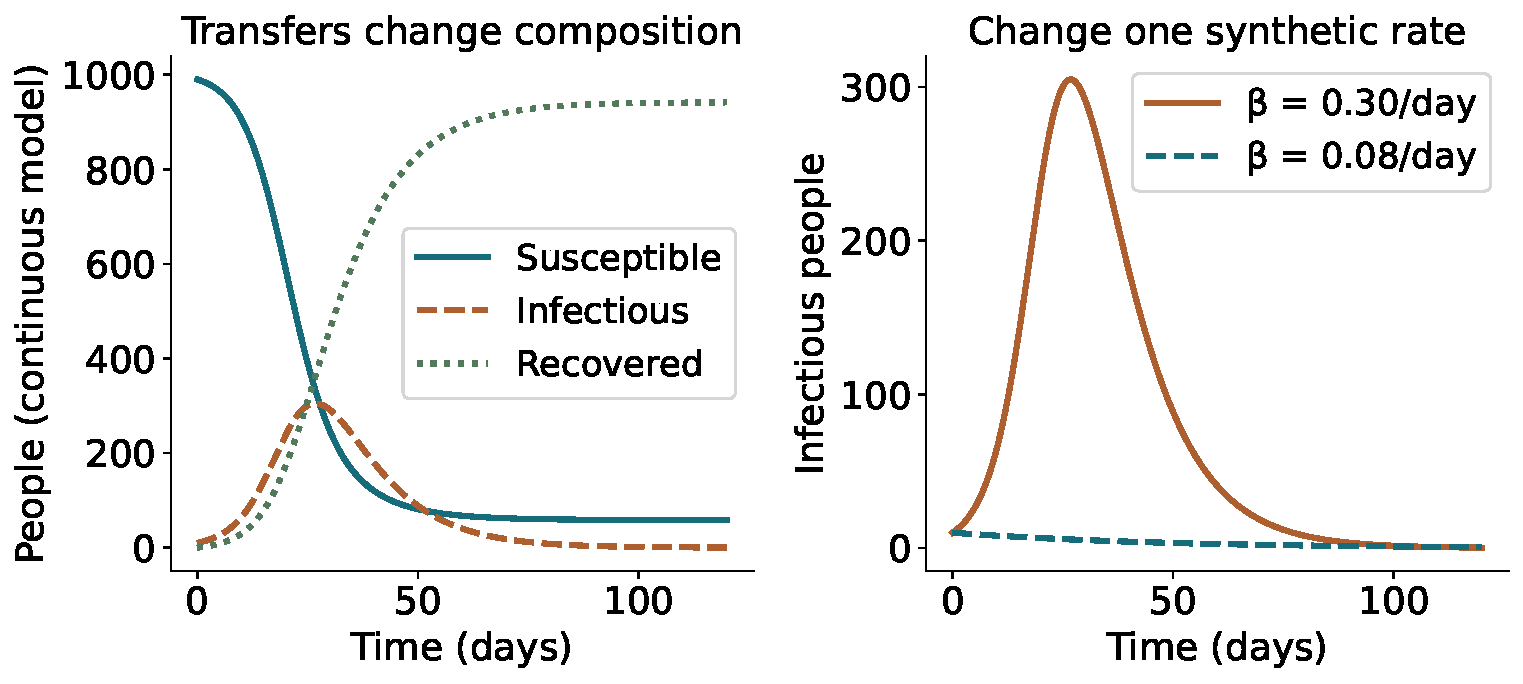
\includegraphics[width=.98\linewidth,height=.69\textheight,keepaspectratio]{population-trajectories.pdf}\end{frame}
\renewcommand{\notestarget}{notes.pdf\#note-growth-threshold-and-the-infectious-peak}
\begin{frame}[t,fragile,label=slide-the-peak-is-a-balance-of-flows]{The peak is a balance of flows}
\[S_p=N\gamma/\beta.\]\pause{} As $S$ falls, infection recruitment eventually falls below recovery.\par\medskip The peak can occur with many susceptible people remaining.
\end{frame}
\renewcommand{\notestarget}{notes.pdf\#note-an-invariant-and-the-final-size-relation}
\begin{frame}[t,fragile,label=slide-eliminating-time-from-two-equations]{Eliminating time from two equations}
\[\frac{\dd I}{\dd S}=\frac{\dot I}{\dot S}=-1+\frac{\gamma N}{\beta S}.\]\pause{} Valid on intervals with $S,I>0$ and $\beta>0$.
\end{frame}
\renewcommand{\notestarget}{notes.pdf\#note-an-invariant-and-the-final-size-relation}
\begin{frame}[t,fragile,label=slide-an-analytic-orbit-relation]{An analytic orbit relation}
\[I-I_0=-(S-S_0)+\frac{\gamma N}{\beta}\log\frac S{S_0}.\]\pause{} The logarithm acts on a dimensionless ratio.\par\medskip This relation checks the trajectory independently of its time parametrization.
\end{frame}
\renewcommand{\notestarget}{notes.pdf\#note-an-invariant-and-the-final-size-relation}
\begin{frame}[t,fragile,label=slide-final-size-and-remaining-susceptibility]{Final size and remaining susceptibility}
\[\log\frac{S_\infty}{S_0}=-\frac\beta{\gamma N}(N-S_\infty-R_0).\]\pause{} Assume $I_\infty=0$ and constant positive parameters.\par\medskip Solve for the trajectory-consistent root; the relation does not force $S_\infty=0$.
\end{frame}
\renewcommand{\notestarget}{notes.pdf\#note-a-conservative-euler-step-and-its-restrictions}
\begin{frame}[t,fragile,label=slide-one-conservative-numerical-step]{One conservative numerical step}
\[\begin{aligned}S^+&=S-hJ_{\mathrm{inf}},\\I^+&=I+h(J_{\mathrm{inf}}-J_{\mathrm{rec}}),\\R^+&=R+hJ_{\mathrm{rec}}.\end{aligned}\]\pause{} Compute each flux once and use it in both affected equations.
\end{frame}
\renewcommand{\notestarget}{notes.pdf\#note-a-conservative-euler-step-and-its-restrictions}
\begin{frame}[t,fragile,label=slide-the-one-day-hand-calculation]{The one-day hand calculation}
\[(990,10,0)\longmapsto(987.03,11.97,1).\]\pause{}\[987.03+11.97+1=1000.\] Two half-steps need not give the same endpoint because their second flux evaluation uses a changed state.
\end{frame}
\renewcommand{\notestarget}{notes.pdf\#note-a-conservative-euler-step-and-its-restrictions}
\begin{frame}[t,fragile,label=slide-a-sufficient-positivity-restriction]{A sufficient positivity restriction}
\[S^+=S(1-h\beta I/N),\qquad I^+=I(1-h\gamma)+h\beta SI/N.\]\pause{}\[h\max(\beta,\gamma)\leq1\] ensures nonnegative states throughout the simplex.
\end{frame}
\renewcommand{\notestarget}{notes.pdf\#note-numerical-evidence-and-model-discrepancy}
\begin{frame}[t,fragile,label=slide-changing-one-transmission-parameter]{Changing one transmission parameter}
For $\beta=0.08$, $\gamma=0.1\ \mathrm{day}^{-1}$:\[\beta S_0/N-\gamma=-0.0208\ \mathrm{day}^{-1}.\]\pause{} Since $S$ cannot increase, infectious prevalence declines from the start.
\end{frame}
\renewcommand{\notestarget}{notes.pdf\#note-numerical-evidence-and-model-discrepancy}
\begin{frame}[t,fragile,label=slide-verification-of-trajectories-and-observables]{Verification of trajectories and observables}
Check $S+I+R$, nonnegativity, monotonic $S,R$, and the analytic orbit.\pause{}\par\medskip Refine $h$ at common times; compare peak height and time separately.\par\medskip Conserved population does not imply an accurate epidemic curve.
\end{frame}
\renewcommand{\notestarget}{notes.pdf\#note-numerical-evidence-and-model-discrepancy}
\begin{frame}[t,fragile,label=slide-evidence-for-a-population-model]{Evidence for a population model}
Document contact assumptions, observation process, initial conditions, and parameter units.\pause{}\par\medskip A continuous hazard and a discrete infection probability are different quantities.\par\medskip Synthetic scenario comparison is not empirical validation.
\end{frame}
\end{document}
